\chapter{Experiments, test and results} % Main chapter title

\label{Chapter 6} % For referencing the chapter elsewhere, use \ref{Chapter1} 

\lhead{Chapter 6. \emph{Experiments, test and results}}

In this chapter, we will present the design of the experiment study in order to validate the proposed solution. The implementation of the experiment is being implemented and is not terminated at the time of this writing.

The main issues behind designing theses experiments were, first, to exercise all aspects of the algorithm (e.g., to find errors in the algorithm design and/or implementation). Next, we want to know how useful might be the technique in a typical application. 


The experimental evaluation was devised in two mains parts, the first consisted on constructing the HTN model to evaluate the Discolog system. The second part consisted to variate the level of knowledge to test the robustness of  Discolog system against different types of breakdown. 


\section{experimental model creation}
In order to test the Discolog system, we had test the Discolog system on different type of HTNs. in the absence of accurate models. we had to create our own evaluation data. Therefore, an algorithm was constructed to generate different types of HTN models. 

The evaluation HTN was constructed using synthetic data as demonstrated in the algorithm \ref{tree}. An example of a (2,2,2) tree is shown in Figure \ref{tree figure}.

\begin{figure}[h]
	\centering
	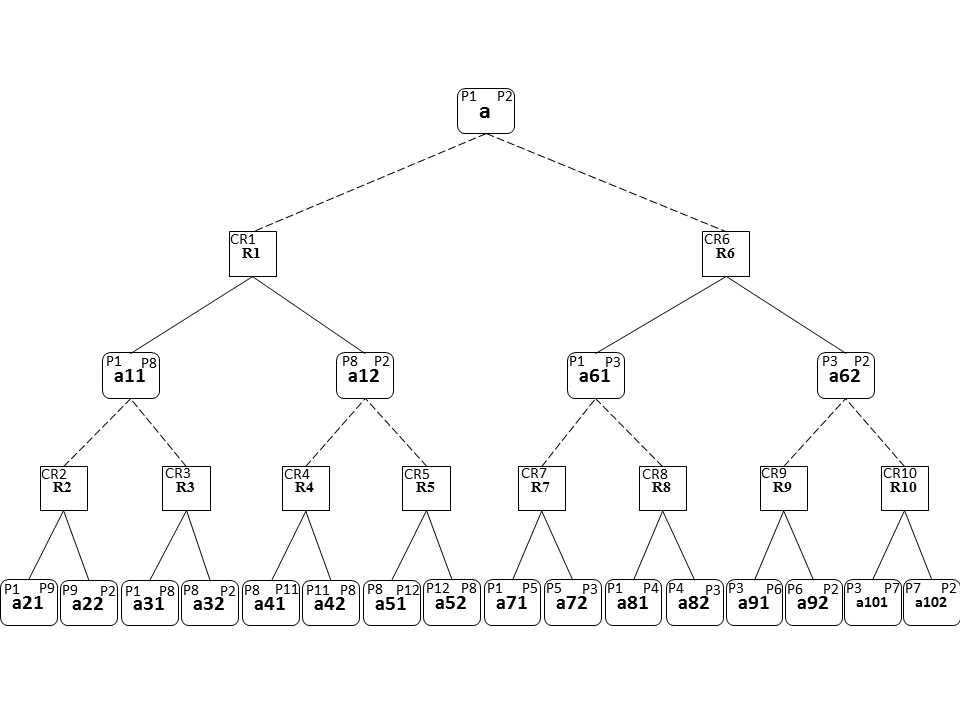
\includegraphics[width=\textwidth]{Pictures/treeg.png}
	\caption{\label{tree figure} Generated tree of depth=2, length=2 and recipes=2}
\end{figure}

\begin{itemize}
	\item Each compound task in the HTN has a set of [$r_1$, ...,$r_\text{recipes}$].
	\item Each recipe is constituted by [$r_1$, ...,$r_\text{length}$] children to decompose the parent task.
	\item the preconditions of the first child are the same as its parent, and the postconditions of the last child are the same as its parent. 
	\item Conditions defined in the primitive tasks are chained in each recipe. Example: the task a is decomposed to \{$a_1$, $a_2$, $a_3$\}using the recipe R1. Thus, the preconditions of $a_1$ are the same as its parent a and the postconditions of $a_3$ are the same as its parent a. We define the postcondition of $a_1$ as "P1" then the preconditions of the next task $a_2$ are "P1", we also define the postconditions of $a_2$ as "P2" then the preconditions of $a_3$ task are "P2".
	\item each recipe has its applicability condition, therefore, we generated primitives tasks whose postconditions turns to true the applicability condition of each recipe, in order to be able to recover from a breakdown caused by an applicability condition failure. 
\end{itemize}
\begin{algorithm}
\caption{Data generation algorithm }\label{tree}
\begin{algorithmic}[]
	\Procedure{CreateHTN}{depth,length,recipes,top}
	\State $\textit{ConstructHTNTree(depth,length,recipes,top)} $

	\State $\textit{DefineLevelOfKnwoledge(top, level)} $
	\EndProcedure \textbf{EndProcedure}
	\State
	\State
	
	\Procedure{ConstructHTNTree}{depth,length,recipes,top}
	\If {$\textit{depth} > 1 $}
\For{$ \textbf{each r} \in \text{ recipes} $}
\State $\text{addRecipe(r, top)}$
\For{$ \textbf{each l} \in \text{ length} $}
\State $\text{addchild(top,childl})$
\State $ConstructHTNTree(depth,length,recipes,childl)$
\EndFor
\EndFor
\EndIf
	\EndProcedure \textbf{EndProcedure}
\end{algorithmic}
\end{algorithm}
\subsection{Test algorithm}
The Discolog system was tested on each generated model several times, and for each model, we variate the type of breakdown to recover from and the level of knowledge used in the model. We calculate the percentage of recover relative to the level of knowledge. The generated algorithm is described bellow.
\begin{algorithm}
	\caption{Test algorithm }\label{test}
	\begin{algorithmic}[]
		\Loop \text{ (10) }
\Loop (\text{Random breakdowns } $\gets$ 100)
\State(Discolog(HTN,Goal))

\EndLoop\textbf{EndLoop} \\
\EndLoop\textbf{EndLoop} \\
	\end{algorithmic}
\end{algorithm}
 
\section{Expected results of the Experiments}

- revoir début pas clair assomption (tu as de la place...)
- expliquer pourquoi cette ppé de monotonie que tu espères avoir dans tes résultats est importante
- expliquer ce qu'il faudrait étudier d'autres (cette expé a des restrictions, il faut les dire, cooking, etc...) validation computationnelle vs...

One of the main purposes of this experiments is to validate our assumption. We assume that the more knowledge we have in the model, the more often we can recover from breakdowns. an graph represented our expected results is shown in Figure \ref{expet}.
As the STRIPS uses the information in the HTN's domain knowledge. Thus, without knowledge in the HTN there is no recover, the same as 100 \% of knowledge assures 100\% of recover. the more information the STRIPS planner get, the more recover plan it can generate.
\begin{figure}[h]
	\centering
	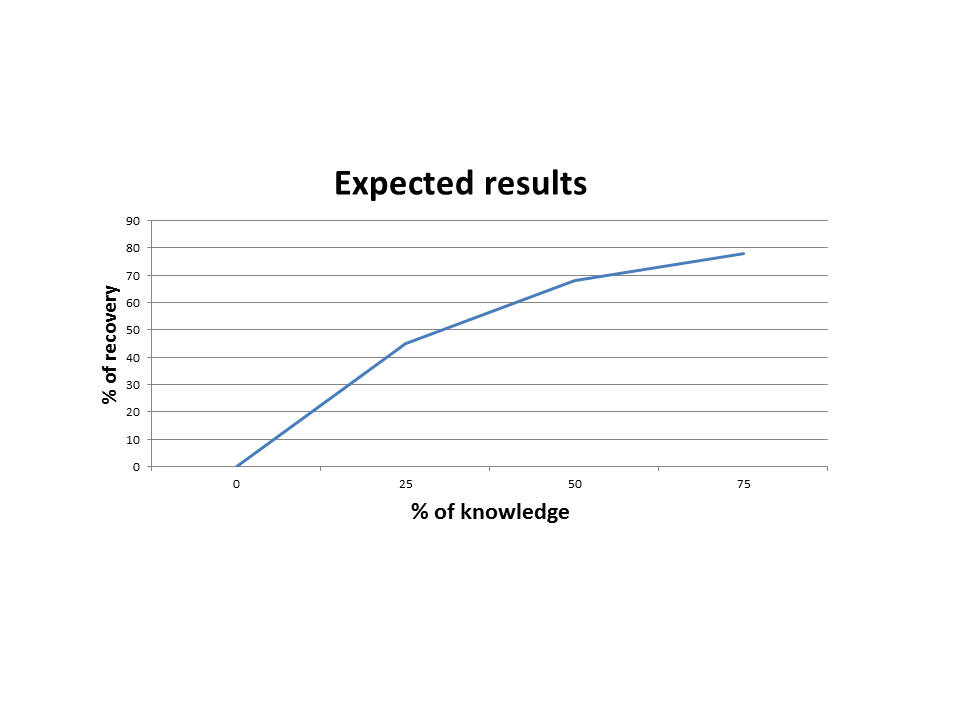
\includegraphics[width=\textwidth]{Pictures/expected.png}
	\caption{\label{expet} The expected experiments results}
\end{figure}

We presented in this Chapter the experiments to evaluate the proposed solution. We discussed the expected results. The month of September will be devoted to the experiments study in order to validate the Discolog system.
